\section{Experiments}
\vspace{-0.05in}

In this section, we conduct a series of experiments to evaluate our model. 
To explore whether the model learns to perform the spatial inference necessary for answering visual questions that explicitly require spatial reasoning, we design a set of experiments using synthetic visual question/answer data in Sec.~\ref{sec:synthetic1}. The experimental results of our model in standard datasets (DAQUAR~\cite{DBLP:journals/corr/MalinowskiF14} and VQA~\cite{DBLP:journals/corr/AntolALMBZP15} datasets) are reported in Sec.~\ref{sec:expstandard}.

%%%%%%%%%%%%%%%%%%%%%%%%%%%%%%%%%%%%%%%%%%%%%%%%%%%%%%%%%%%%%%%%%%%%%%%%%%%%%%%%%%%%%%%%%%%%%%%%%%%
\subsection{Exploring Attention on Synthetic Data}\label{sec:synthetic1}
%Several public datasets are available, however, 
The questions in the public VQA datasets are quite varied and difficult and often require common sense knowledge to answer (e.g., ``Does this man have 20/20 vision?'' about a person wearing glasses). Furthermore, past work~\cite{malinowski2015ask,DBLP:journals/corr/RenKZ15} showed that the question text alone (no image) is a very strong predictor of the answer.
Therefore, before evaluating on standard datasets, we would first like to
understand how the proposed model uses spatial attention to answer simple visual questions where the answer cannot be predicted from question alone. 
Our visualization demonstrates that the attention mechanism does learn to attend to objects and gather evidence via certain inference rules. 

%%%%%%%%%%% figure
\begin{figure*}[!t]
  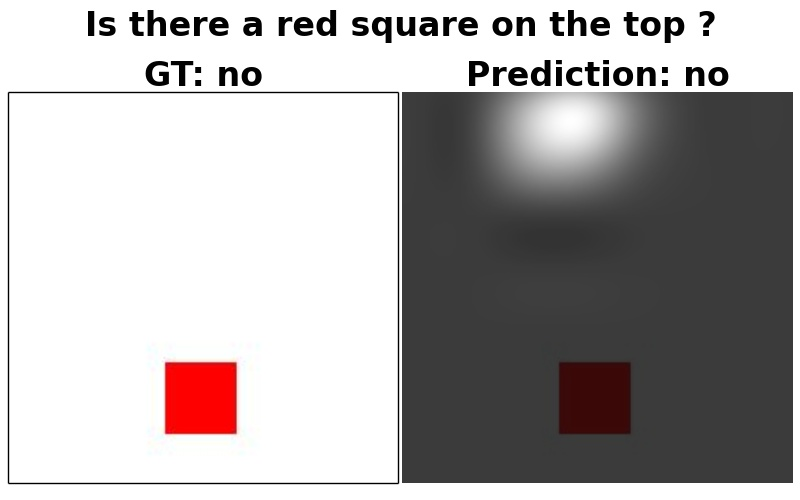
\includegraphics[width=0.242\textwidth]{figures/rule1_im_30075_219_top.JPEG}
  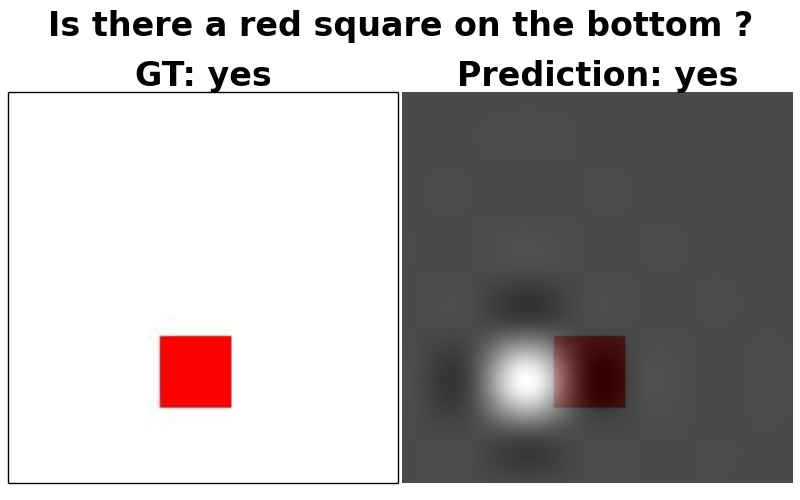
\includegraphics[width=0.242\textwidth]{figures/rule1_im_31186_4441_bottom.JPEG}
  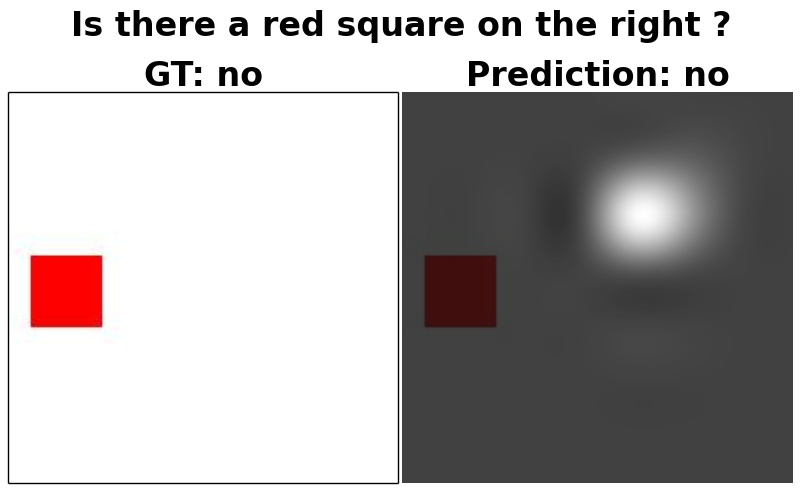
\includegraphics[width=0.242\textwidth]{figures/rule1_im_31189_690_right.JPEG}
  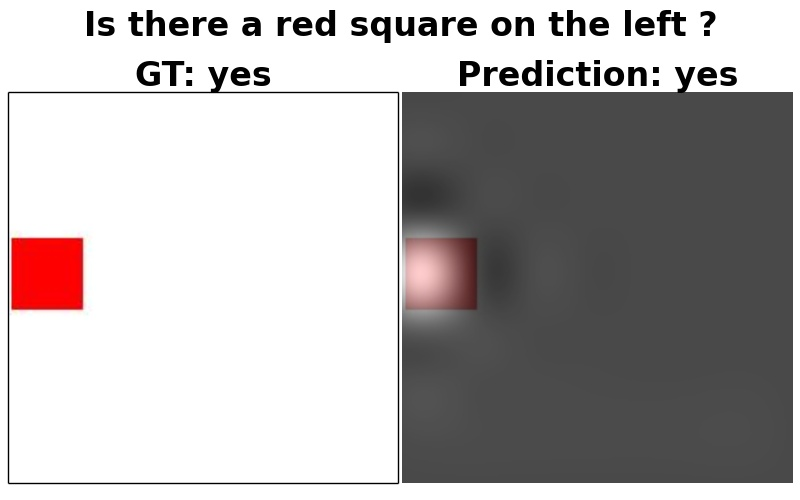
\includegraphics[width=0.242\textwidth]{figures/rule1_im_31200_4217_left.JPEG}\\
  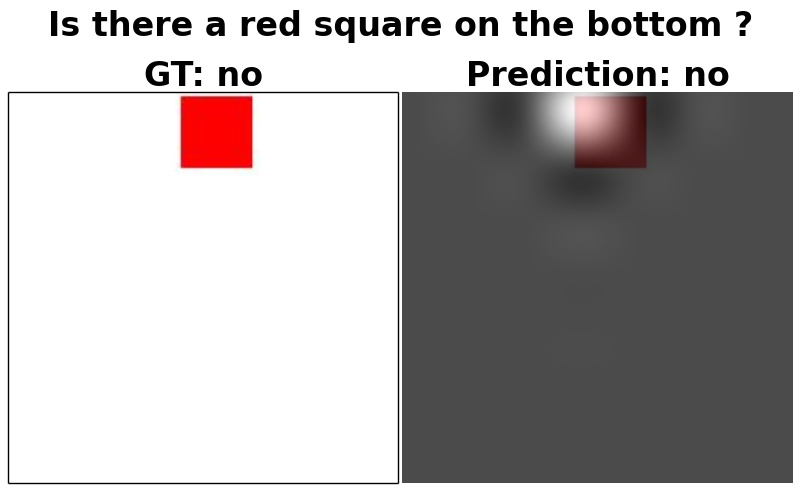
\includegraphics[width=0.242\textwidth]{figures/rule2_im_30004_3495_bottom.JPEG}
  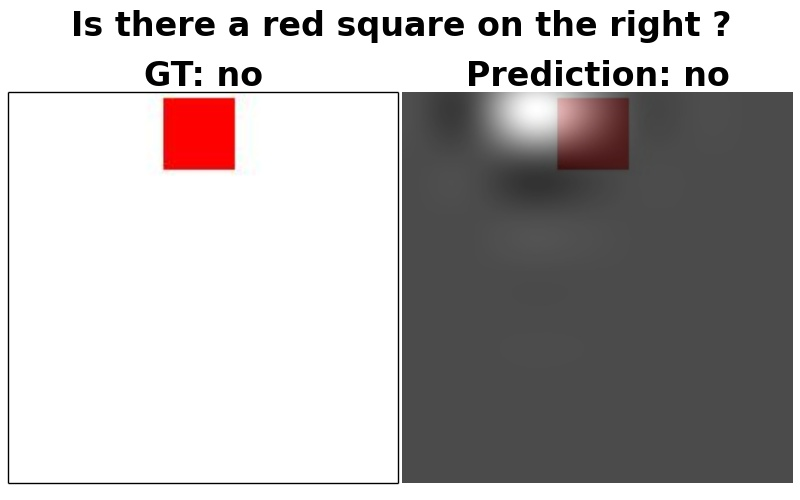
\includegraphics[width=0.242\textwidth]{figures/rule2_im_30036_3165_right.JPEG}
  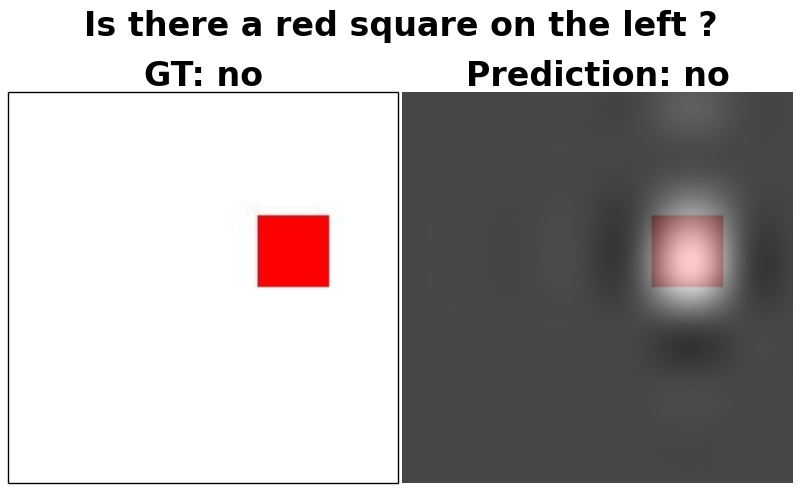
\includegraphics[width=0.242\textwidth]{figures/rule2_im_31185_2199_left.JPEG}
  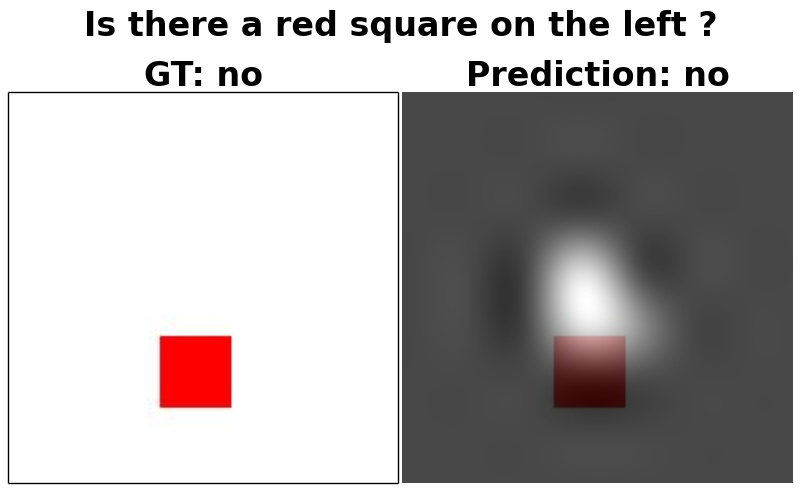
\includegraphics[width=0.242\textwidth]{figures/rule2_im_31186_1310_left.JPEG}
%\includegraphics[width=\textwidth]{figures/onehop_twohop.png}
\vspace{-0.1in}
\caption{\textbf{Absolute position experiment:} for each image and question pair, we show the original image (left) and the attention weights $W_{att}$ (right). 
The attention follows the following rules. The first rule (top row) looks at the position specified in question (top$\mid$bottom$\mid$right$\mid$left), if it contains a square, answer ``yes''; otherwise answer ``no''.
The second rule (bottom row) looks at the region where there is a square, and answers ``yes'' if the question contains that position and ``no'' for the other three positions.}\label{fig:red_square}
\vspace{-0.1in}
\end{figure*}


%%%%%%%%%%%%%%%%%%%%%%%%%%%%%%%%%%%%%%%%%%%%%%%%%%%%%%%%%%%%%%%%%%%%%%%%%%%%%%%%%%%%%%%%%%%%%%%%%%%
\vspace{-0.1in}
\subsubsection{Absolute Position Recognition}\label{sec:absolute}
We investigate whether the model has the ability to recognize the absolute location of the object in the image. We explore this by designing a simple task where an object (a red square) appears in some region of a white-background image, and the question is ``Is there a red square on the [top$\mid$bottom$\mid$left$\mid$right]?'' For each image, we randomly place the square in one of the four regions, and generate the four questions above, together with three ``no'' answers and one ``yes'' answer. The generated data is split into training and testing sets. 

Due to the simplicity of this synthetic dataset, the SMem-VQA one-hop model achieves 100\% test accuracy. However, the baseline model (iBOWIMG)~\cite{zhou2015simple} cannot infer the answer and only obtains accuracy of around 75\%, which is the prior probability of the answer ``no'' in the training set. The SMem-VQA one-hop model is equivalent to the iBOWIMG model if the attention weights in our one-hop model are set equally for each location, since the iBOWIMG model uses the mean pool of the convolutional feature ($inception\_5b/output$) in GoogLeNet that we use in SMem-VQA model. 
We check the visualization of the attention weights and find that the relationship between the high attention position and the answer can be expressed by logical expressions.
We show the attention weights of several typical examples in Fig.~\ref{fig:red_square} which reflect two logic rules:
1)~Look at the position specified in question (top$\mid$bottom$\mid$right$\mid$left), if it contains a square, then answer ``yes''; if it does not contain a square, then answer ``no''.
2)~Look at the region where there is a square, then answer ``yes'' for the question about that position and ``no'' for the questions about the other three positions.

In the iBOWIMG model, the mean-pooled GoogLeNet visual features lose spatial information and thus cannot distinguish images with a square in different positions. On the contrary, our SMem-VQA model can pay high attention to different regions according to the question, and generate an answer based on the selected region, using some learned inference rules.
This experiment demonstrates that the attention mechanism in our model is able to make absolute spatial location inference based on the spatial attention. 


%%%%%%%%%%% figure
\begin{figure*}[t]
  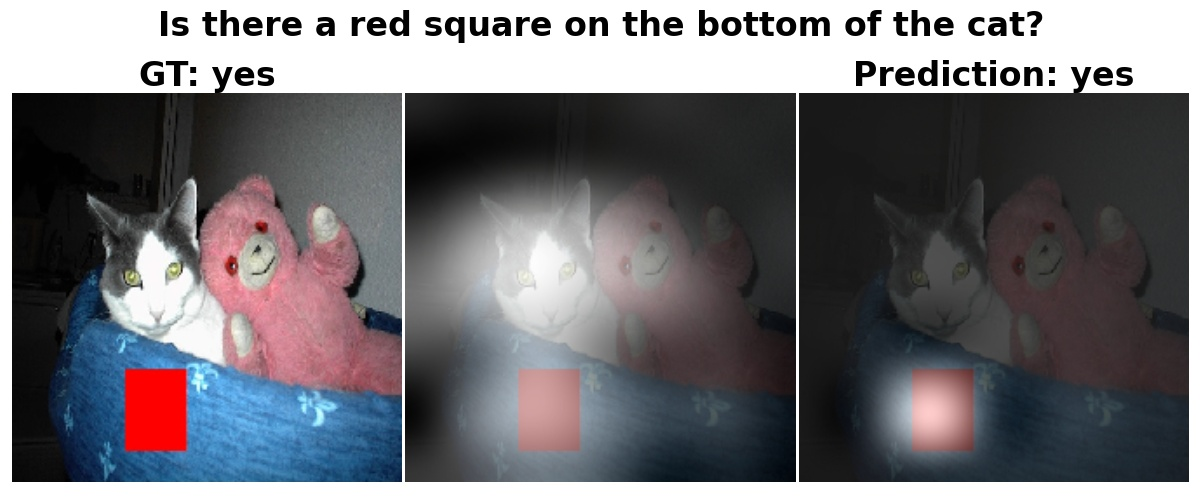
\includegraphics[width=0.325\textwidth]{figures/bottom_COCO_val2014_000000167602_bottom.jpg}
  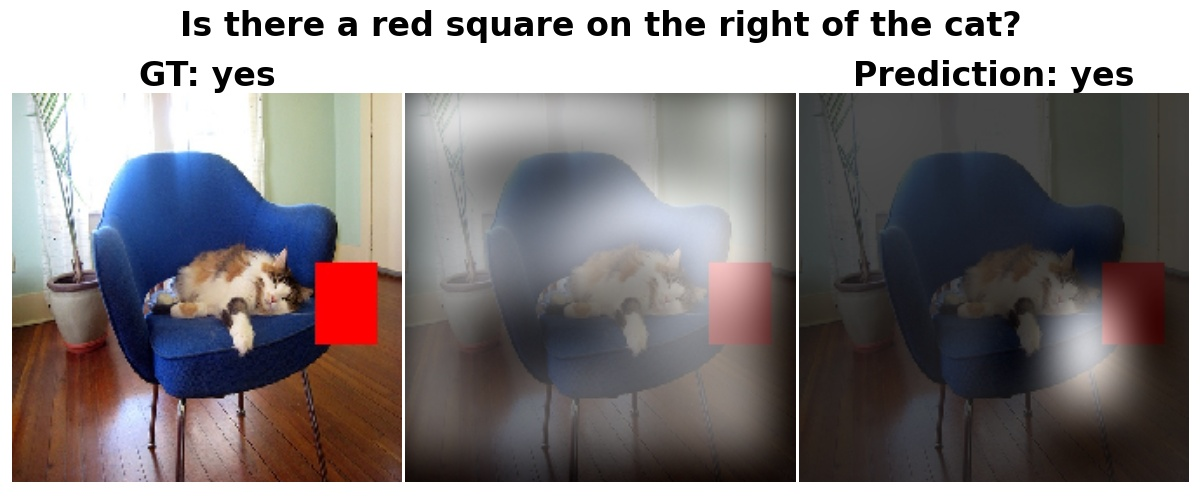
\includegraphics[width=0.325\textwidth]{figures/right_COCO_val2014_0000002988_right.jpg}
  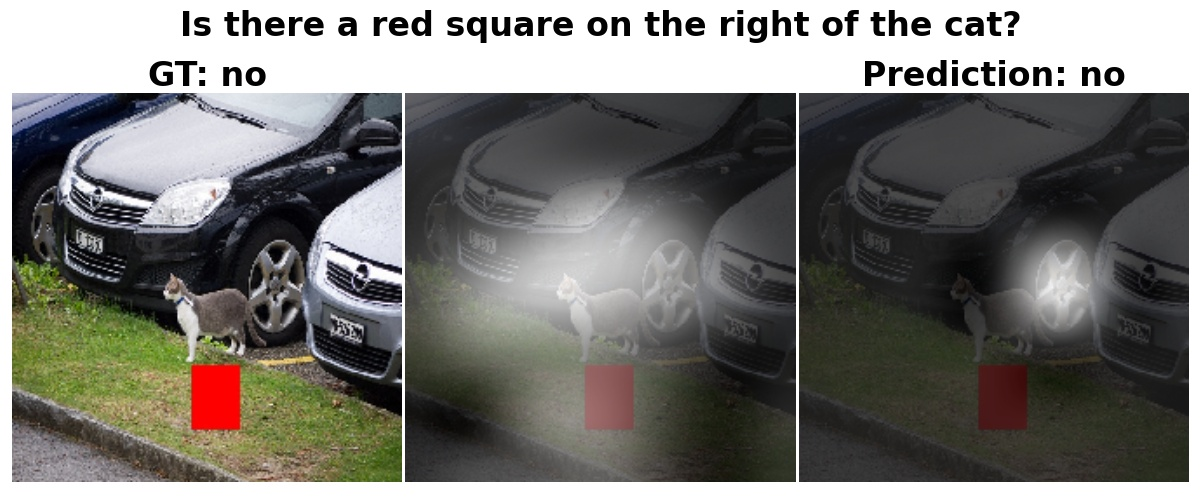
\includegraphics[width=0.325\textwidth]{figures/right_COCO_val2014_000000172330_bottom.jpg}\\
  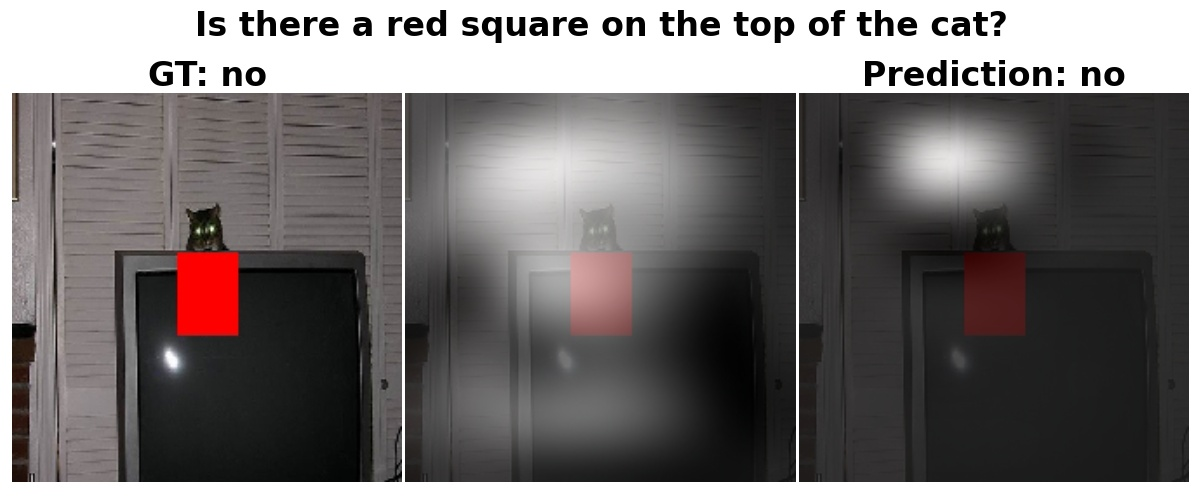
\includegraphics[width=0.325\textwidth]{figures/top_COCO_val2014_00000010694_bottom}
  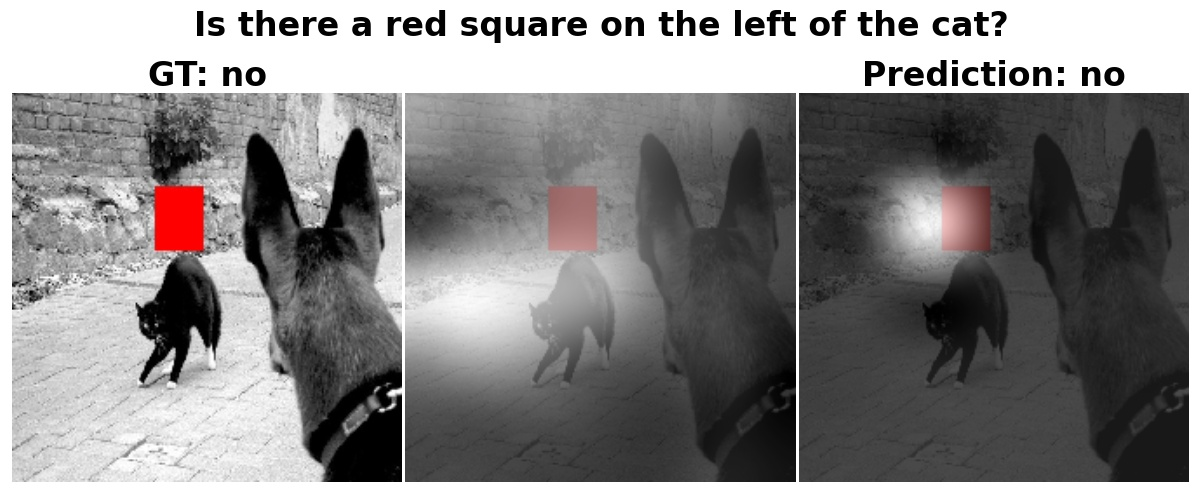
\includegraphics[width=0.325\textwidth]{figures/left_COCO_val2014_000000201918_top.jpg}
  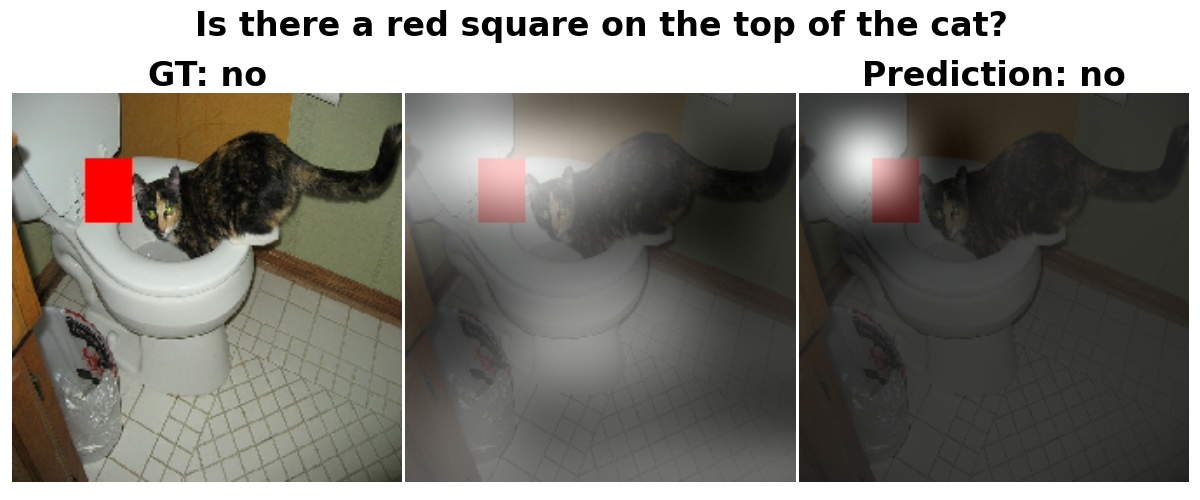
\includegraphics[width=0.325\textwidth]{figures/top_COCO_val2014_000000218924_left.jpg}
\vspace{-0.05in}
\caption{\textbf{Relative position experiment:}
for each image and question pair, we show the original image (left), the evidence embedding $W_E$ of the convolutional layer (middle) and the attention weights $W_{att}$ (right). The evidence embedding $W_E$ has high activations on both cat and red square. 
The attention weights follow similar inference rules as in Fig.~\ref{fig:red_square}, with the difference that the attention position is around the cat.
%Rule#1: (top row) look at the specified position (top/bottom/right/left), if it contains a square, answer "yes"; otherwise answer "no".
%Rule#2: (bottom row) look at the region where there is a square, answer "yes" if the question contains that position and "no" if it contains one of the other three positions.
}\label{fig:cat_square}
\vspace{-0.2in}
\end{figure*}


%%%%%%%%%%%%%%%%%%%%%%%%%%%%%%%%%%%%%%%%%%%%%%%%%%%%%%%%%%%%%%%%%%%%%%%%%%%%%%%%%%%%%%%%%%%%%%%%%%%
\vspace{-0.1in}
\subsubsection{Relative Position Recognition}
In order to check whether the model has the ability to infer the  position of one object \textit{relative} to another object,
we collect all the cat images from the MS COCO Detection dataset~\cite{lin2014microsoft}, and add a red square on the [top$\mid$bottom$\mid$left$\mid$right] of the bounding box of the cat in the images.
For each generated image, we create four questions, ``Is there a red square on the [top$\mid$bottom$\mid$left$\mid$right] of the cat?'' together with three ``no'' answers and one ``yes'' answer. 
We select 2639 training cat images and 1395 testing cat images from MS COCO Detection dataset. 

Our SMem-VQA one-hop model achieves 96\% test accuracy on this synthetic task, while the baseline model (iBOWIMG) accuracy is around 75\%.
We also check that another simple baseline that predicts the answer based on the absolute position of the square in the image gets around 70\% accuracy. 
We visualize the evidence embedding $W_E$ features and the attention weights $W_{att}$ of several typical examples in Fig.~\ref{fig:cat_square}.
The evidence embedding $W_E$ has high activations on the cat and the red square, while the attention weights pay high attention to certain locations around the cat.
We can analyze the attention in the correctly predicted examples using the same rules as in absolute position recognition experiment. 
These rules still work, but the position is relative to the cat object:
1)~Check the specified position relative to the cat, if it finds the square, then answer ``yes'', otherwise ``no''; 2)~Find the square, then answer ``yes'' for the specified position, and answer ``no'' for the other positions around the cat.
We also check the images where our model makes mistakes, and find that the mistakes mainly occur in images with more than one cats. The red square appears near only one of the cats in the image, but our model might make mistakes by focusing on the other cats.
We conclude that our SMem-VQA model can infer the relative spatial position based on the spatial attention around the specified object, which can also be represented by some logical inference rules. 



%%%%%%%%%%%%%%%%%%%%%%%%%%%%%%%%%%%%%%%%%%%%%%%%%%%%%%%%%%%%%%%%%%%%%%%%%%%%%%%%%%%%%%%%%%%%%%%%%%%
%%%%%%%%%%%%%% table
\begin{table}[!t]
\centering
\caption{Accuracy results on the DAQUAR dataset (in percentage).}
\small
 \begin{tabular}{l || c c c} 
 \hline
 ~ & DAQUAR\\ \hline
 Multi-World~\cite{DBLP:journals/corr/MalinowskiF14} & 12.73 \\ %\hline
 Neural-Image-QA~\cite{malinowski2015ask} & 29.27  \\ %\hline
 Question LSTM~\cite{malinowski2015ask} & 32.32 \\ %\hline
 VIS+LSTM~\cite{DBLP:journals/corr/RenKZ15} & 34.41 \\ %\hline
 Question BOW~\cite{DBLP:journals/corr/RenKZ15} & 32.67 \\ %\hline
 IMG+BOW~\cite{DBLP:journals/corr/RenKZ15} & 34.17 \\ \hline
 %2-VIS+BLSTM ~\cite{DBLP:journals/corr/RenKZ15} &  - & 35.78  & -\\ \hline \hline
 %Question One-Hop & 53.37 & 36.03 & - \\ %\hline   
 SMem-VQA One-Hop & 36.03 \\ %\hline   
 SMem-VQA Two-Hop & \bf{40.07} \\ \hline 
 %one dimension convolution hierarchy model\cite{ma2015learning} &  - & 0.3933 \cite{ma2015learning} & - \\ \hline
 \end{tabular}
\label{fig:baseline}
\vspace{-0.2in}
\end{table}


\subsection{Experiments on Standard Datasets}\label{sec:expstandard}
%\vspace{-0.08in}
\subsubsection{Results on DAQUAR}
The DAQUAR dataset is a relatively small dataset which builds on the NYU Depth Dataset V2~\cite{Silberman:ECCV12}. We use the reduced DAQUAR dataset~\cite{DBLP:journals/corr/MalinowskiF14}. The evaluation metric for this dataset is 0-1 accuracy. 
The embedding dimension is 512 for our models running on the DAQUAR dataset. 
We use several reported models on DAQUAR as baselines, which are listed below:\\
%\noindent
{$\bullet$} {\bf{Multi-World}}~\cite{DBLP:journals/corr/MalinowskiF14}: an approach based on handcrafted features using a semantic parse of the question and scene analysis of the image combined in a latent-world Bayesian framework.\\ 
{$\bullet$} {\bf{Neural-Image-QA}}~\cite{malinowski2015ask}: uses an LSTM to encode the question and then decode the hidden information into the answer. The image CNN feature vector is shown at each time step of the encoding phase.\\
{$\bullet$} {\bf{Question LSTM}}~\cite{malinowski2015ask}: only shows the question to the LSTM to predict the answer without any image information.\\
{$\bullet$} {\bf{VIS+LSTM}}~\cite{DBLP:journals/corr/RenKZ15}: similar to Neural-Image-QA, but only shows the image features to the LSTM at the first time step, and the question in the remaining time steps to predict the answer.\\
{$\bullet$} {\bf{Question BOW}}~\cite{DBLP:journals/corr/RenKZ15}: only uses the BOW question representation and a single hidden layer neural network to predict the answer, without any image features.\\
{$\bullet$} {\bf{IMG+BOW}}~\cite{DBLP:journals/corr/RenKZ15}: concatenates the BOW question representation with image features, and then uses a single hidden layer neural network to predict the answer. This model is similar to the iBOWIMG baseline model in~\cite{zhou2015simple}.

Results of our SMem-VQA model on the DAQUAR dataset and the baseline model results reported in previous work are shown in Tab.~\ref{fig:baseline}. 
From the DAQUAR result in Tab.~\ref{fig:baseline}, we see that models based on deep features significantly outperform the Multi-World approach based on hand-crafted features. Modeling the question only with either the LSTM model or Question BOW model does equally well in comparison, indicating the the question text contains important prior information for predicting the answer. Also, on this dataset, the VIS+LSTM model achieves better accuracy than Neural-Image-QA model; the former shows the image only at the first timestep of the LSTM, while the latter does so at each timestep. In comparison, both our One-Hop model and Two-Hop spatial attention models outperform the IMG+BOW, as well as the other baseline models.
A major advantage of our model is the ability to visualize the inference process in the deep network. To illustrate this, two attention weights visualization examples in SMem-VQA One-Hop and Two-Hop models on DAQUAR dataset are shown in Fig.~\ref{fig:2hopVQA} (bottom row).



%%%%%%%%%%% figure
\begin{figure*}[t]
%  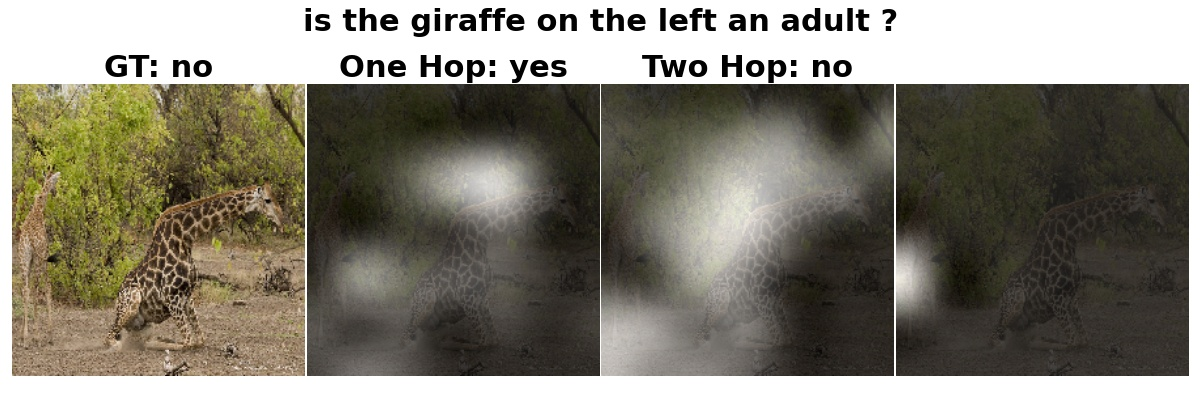
\includegraphics[width=0.5\textwidth]{figures/VQA-DAQUAR_One-Hop_Two-Hop/COCO_val2014_000000014271.jpg}
%  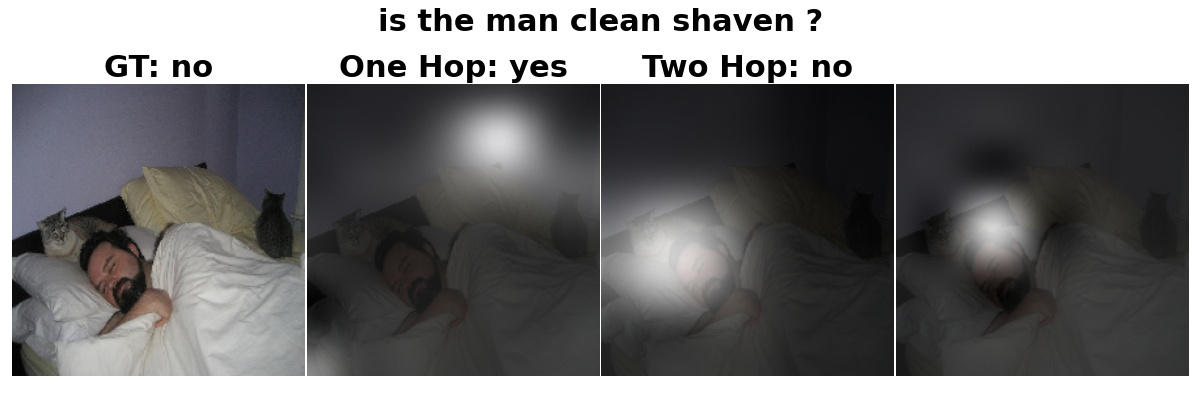
\includegraphics[width=0.5\textwidth]{figures/VQA-DAQUAR_One-Hop_Two-Hop/COCO_val2014_000000012085.jpg}\\
  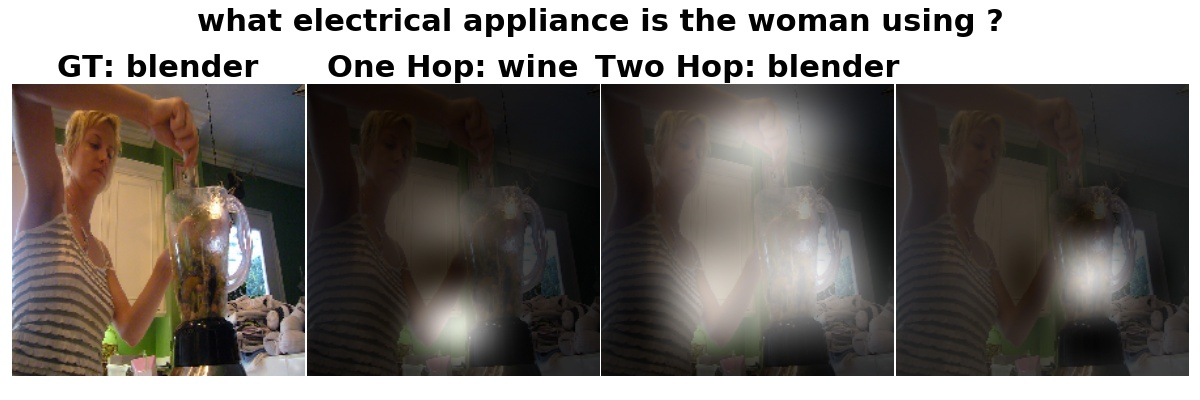
\includegraphics[width=0.5\textwidth]{figures/VQA-DAQUAR_One-Hop_Two-Hop/CO_train2014_000000575060_5750602.jpg}
  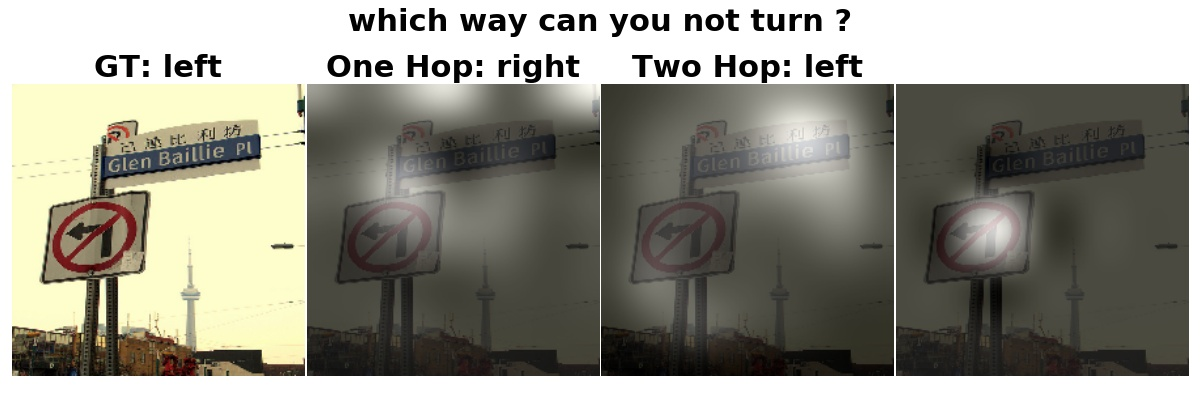
\includegraphics[width=0.5\textwidth]{figures/VQA-DAQUAR_One-Hop_Two-Hop/CO_train2014_000000222383_2223830.jpg}\\
  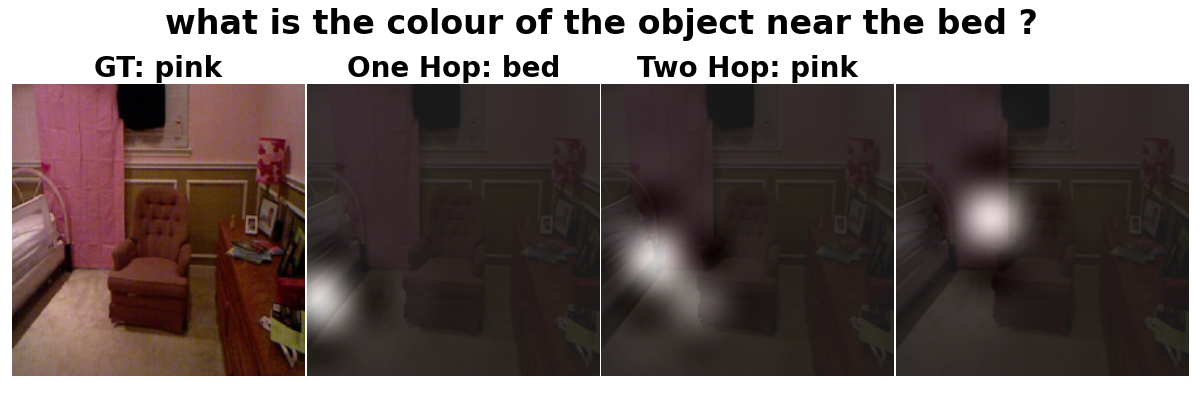
\includegraphics[width=0.5\textwidth]{figures/VQA-DAQUAR_One-Hop_Two-Hop/image1183.png}
  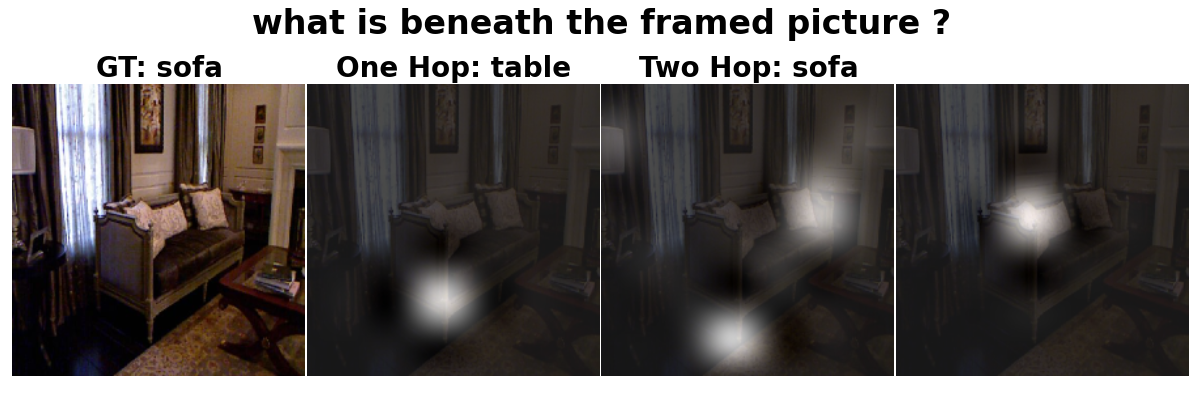
\includegraphics[width=0.5\textwidth]{figures/VQA-DAQUAR_One-Hop_Two-Hop/image1444.png}
\vspace{-0.25in}
\caption{Visualization of the spatial attention weights in the SMem-VQA One-Hop and Two-Hop models on VQA (top row) and DAQUAR (bottom row) datasets. For each image and question pair, we show the original image, the attention weights $W_{att}$ of the One-Hop model, and the two attention weights $W_{att}$ and $W_{att2}$ of the Two-Hop model in order.}\label{fig:2hopVQA}
\vspace{-0.15in}
\end{figure*}
% \vspace{-0.1in}
\subsubsection{Results on VQA}

The VQA dataset is a recent large dataset based on MS COCO~\cite{lin2014microsoft}. We use the full release (V1.0) open-ended dataset, which contains a train set and a val set. Following standard practice, we choose the top 1000 answers in train and val sets as possible prediction answers, and only keep the examples whose answers belong to these 1000 answers as training data. The question vocabulary size is 7477 with the word frequency of at least three.
Because of the larger training size, the embedding dimension is 1000 on the VQA dataset.
We report the test-dev and test-standard results from the VQA evaluation server.
The server evaluation uses the evaluation metric introduced by~\cite{DBLP:journals/corr/AntolALMBZP15}, which gives partial credit to certain synonym answers:
%\begin{equation}
%Acc({\color{red}ans}) = \min\left\{ \frac{\text{\# human that said }{\color{red} ans}}{3},1\right\}
%$Acc({ans}) = \min\left\{ \frac{\text{\# humans that said }{ans}}{3},1\right\}$.
$Acc({ans}) = \min\left\{ (\text{\# humans that said }{ans})/3,1\right\}$.
%\end{equation}


For the attention models, we do not mirror the input image when using the CNN to extract convolutional features, since this might cause confusion about the spatial locations of objects in the input image.
%The input image size for CNN is $224 \times 224$.
The optimization algorithm used is stochastic gradient descent (SGD) with a minibatch of size 50 and momentum of 0.9.
The base learning rate is set to be 0.01 which is halved every six epoches. Regularization, dropout and L2 norm are cross-validated and used. 


%%%%%%%%%%%%%% another candidate table with test-standard
\begin{table}[!t]
\centering
\caption{Test-dev and test-standard results on the Open-Ended VQA dataset (in percentage). Models with ${}^\ast$ use external training data in addition to the VQA dataset.}
\scriptsize
 \begin{tabular}{l || c c c c || c c c c} 
 \hline
 ~ & \multicolumn{4}{c||}{test-dev}  & \multicolumn{4}{c}{test-standard}\\ 
 ~ & \bf{Overall}  & yes/no  & number  & others & \bf{Overall}  & yes/no  & number  & others\\ \hline
 LSTM Q+I~\cite{DBLP:journals/corr/AntolALMBZP15} & 53.74 & 78.94  & 35.24  & 36.42 & 54.06 & -  & -  & -\\ %\hline
 ACK${}^\ast$~\cite{wu2015ask} & 55.72 & 79.23  & 36.13  & 40.08 & 55.98 & 79.05  & 36.10  & 40.61\\ %\hline
 DPPnet${}^\ast$~\cite{noh2015image} & 57.22 & 80.71  & 37.24  & 41.69 & 57.36 & 80.28  & 36.92  & 42.24\\ %\hline
 iBOWIMG~\cite{zhou2015simple} & 55.72 & 76.55  & 35.03  & 42.62 & 55.89 & 76.76  & 34.98  & 42.62\\ \hline 
 SMem-VQA One-Hop & 56.56 & 78.98 & 35.93  & 42.09 & - & -  & -  & -\\ %\hline   
 SMem-VQA Two-Hop & \textbf{57.99} & \textbf{80.87}  & \textbf{37.32}  & \textbf{43.12} & \textbf{58.24} & \textbf{80.8}  & \textbf{37.53}  & \textbf{43.48}\\ \hline 
 \end{tabular}
\label{fig:baseline2}
\vspace{-0.15in}
\end{table}

For the VQA dataset, we use the simple iBOWIMG model in~\cite{zhou2015simple} as one baseline model, which beats most existing VQA models currently on arxiv.org. We also compare to two models in~\cite{wu2015ask}\cite{noh2015image} which have comparable or better results to the iBOWIMG model. These three baseline models as well the best model in VQA dataset paper~\cite{DBLP:journals/corr/AntolALMBZP15} are listed in the following:\\
%\noindent
{$\bullet$} {\bf{LSTM Q+I}}~\cite{DBLP:journals/corr/AntolALMBZP15}: uses the element-wise multiplication of the LSTM encoding of the question and the image feature vector to predict the answer. This is the best model in the VQA dataset paper.\\
{$\bullet$} {\bf{ACK}}~\cite{wu2015ask}: shows the image attribute features, the generated image caption and relevant external knowledge from knowledge base to the LSTM at the first time step, and the question in the remaining time steps to predict the answer.\\
{$\bullet$} {\bf{DPPnet}}~\cite{noh2015image}: uses the Gated Recurrent Unit (GRU) representation of question to predict certain parameters for a CNN classification network. They pre-train the GRU for question representation on a large-scale text corpus to improve the GRU generalization performance.\\
{$\bullet$} {\bf{iBOWIMG}}~\cite{zhou2015simple}: concatenates the BOW question representation with image feature (GoogLeNet), and uses a softmax classification to predict the answer. 

The overall accuracy and per-answer category accuracy for our SMem-VQA models and the four baseline models on VQA dataset are shown in Tab.~\ref{fig:baseline2}. From the table, we can see that the SMem-VQA One-Hop model obtains slightly better results compared to the iBOWIMG model. However, the SMem-VQA Two-Hop model achieves an improvement of 2.27\% on test-dev and 2.35\% on test-standard compared to the iBOWIMG model, demonstrating the value of spatial attention. The SMem-VQA Two-Hop model also shows best performance in the per-answer category accuracy. 
The SMem-VQA Two-Hop model has slightly better result than the DPPnet model. 
The DPPnet model uses a large-scale text corpus to pre-train the Gated Recurrent Unit (GRU) network for question representation.
Similar pre-training work on extra data to improve model accuracy has been done in~\cite{venugopalan2014translating}.
Considering the fact that our model does not use extra data to pre-train the word embeddings, its results are very competitive.
We also experiment with adding a third hop into our model on the VQA dataset, but the result does not improve further.

The attention weights visualization examples for the SMem-VQA One-Hop and Two-Hop models on the VQA dataset are shown in Fig.~\ref{fig:2hopVQA} (top row). From the visualization, we can see that the two-hop model collects supplementary evidence for inferring the answer, which may be necessary to achieve an improvement on these complicated real-world datasets. We also visualize the fine-grained alignment in the first hop of our SMem-VQA Two-Hop model in Fig.~\ref{fig:VQA_hop1Atten_wordAtten}. 
%through visualizing the attention weights and the correlation value vector from the correlation matrix $C$ for the location with highest attention weight
The correlation vector values (blue bars) measure the correlation between image regions and each word vector in the question. Higher values indicate stronger correlation of that particular word with the specific location's image features. We observe that the fine-grained visual evidence collected using each local word vector, together with the global visual evidence from the whole question, complement each other to infer the correct answer for the given image and question, as shown in Fig.~\ref{fig:concept}.


%%%%%%%%%%% figure
\begin{figure*}[t]
  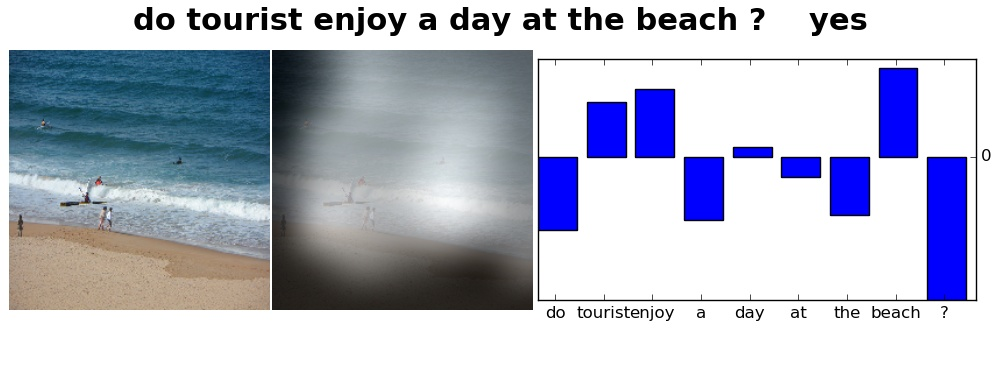
\includegraphics[width=0.5\textwidth]{figures/word_atten/COCO_val2014_000000540932_5409320.jpg}
  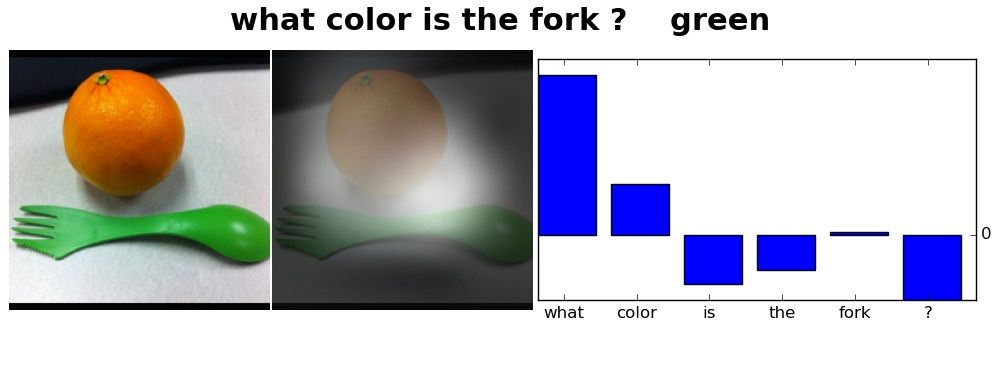
\includegraphics[width=0.5\textwidth]{figures/word_atten/COCO_val2014_000000563730_5637302.jpg}\\
  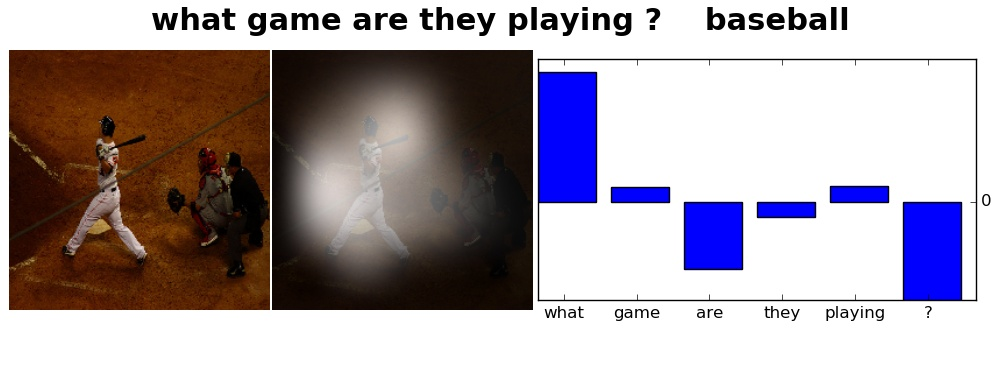
\includegraphics[width=0.5\textwidth]{figures/word_atten/COCO_val2014_000000576875_5768752.jpg}
  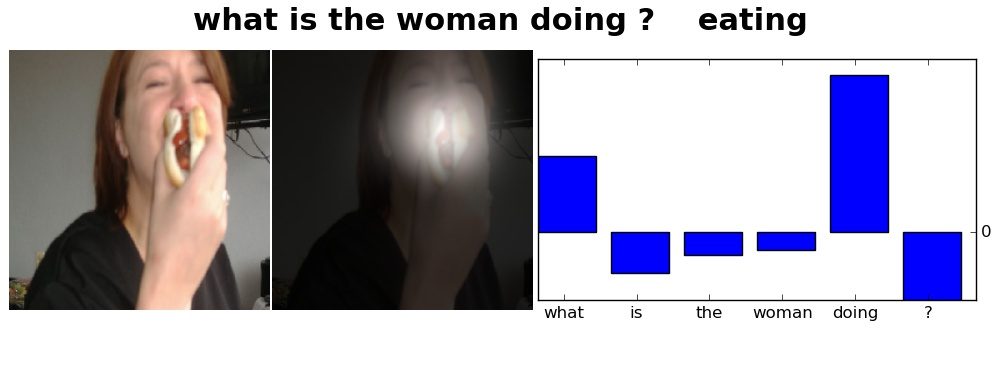
\includegraphics[width=0.5\textwidth]{figures/word_atten/COCO_val2014_000000567340_5673401.jpg}
\vspace{-0.3in}
\caption{
Visualization of the original image (left), the spatial attention weights $W_{att}$ in the first hop (middle) and one correlation vector from the correlation matrix $C$ for the location with highest attention weight in the SMem-VQA Two-Hop model on the VQA dataset.
Higher values in the correlation  vector indicate  stronger correlation of that word with the chosen location's image features.}
\label{fig:VQA_hop1Atten_wordAtten}
\vspace{-0.15in}
\end{figure*}




 





